\setauthor{\secondauthor}

LearnHub unterstützt Schüler:innen und Lehrkräfte der HTL Leonding 
bei der Maturavorbereitung. Das System besteht aus drei zentralen 
Funktionsbereichen: dem \textbf{Maturaupload} für die Verwaltung 
von Mitschriften, dem \textbf{Fragenkonfigurator} für das Erstellen 
und Verwalten von Fragen sowie dem \textbf{Lernmodus} zum Üben und 
Wiederholen. Die folgenden Abbildungen zeigen die Use-Cases der 
einzelnen Funktionsbereiche.


\setauthor{\firstauthor}

\begin{figure}[H]
\centering
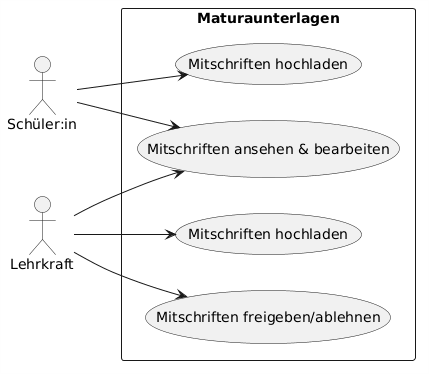
\includegraphics[width=0.75\textwidth]{pics/usecase_maturaunterlagen.png}
\caption{Use-Case-Diagramm: Maturaunterlagen}
\label{fig:ucd_maturaunterlagen}
\end{figure}

Der Maturaupload ermöglicht Schüler:innen das Hochladen und Einsehen 
von Mitschriften. Lehrkräfte können Mitschriften freigeben oder ablehnen 
sowie alle Mitschriften verwalten.

\begin{figure}[H]
\centering
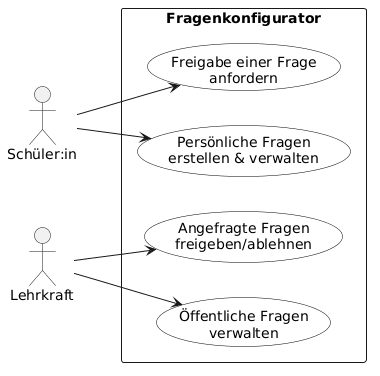
\includegraphics[width=0.75\textwidth]{pics/usecase_fragenkonf.png}
\caption{Use-Case-Diagramm: Fragenkonfigurator}
\label{fig:ucd_fragenkonfigurator}
\end{figure}

Der Fragenkonfigurator erlaubt Schüler:innen das Erstellen privater 
Fragen sowie das Anfordern einer Freigabe. Lehrkräfte verwalten 
öffentliche Fragen und entscheiden über angefragte Freigaben.

\begin{figure}[H]
\centering
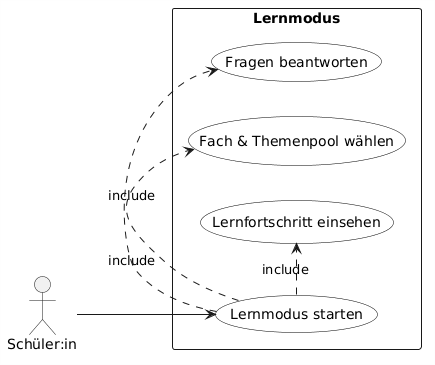
\includegraphics[width=0.75\textwidth]{pics/usecase_lernmodus.png}
\caption{Use-Case-Diagramm: Lernmodus}
\label{fig:ucd_lernmodus}
\end{figure}

Im Lernmodus können Schüler:innen gezielt nach Fach und Themenpool 
filtern, Fragen beantworten und ihren Lernfortschritt einsehen.




\setauthor{\secondauthor}
Das System unterscheidet zwischen zwei Rollen: Schüler:innen 
und Lehrkräfte. Beide Rollen haben Zugriff auf die Plattform, 
unterscheiden sich aber deutlich in ihren Berechtigungen.

\textbf{Schüler:innen} können eigene Mitschriften hochladen und 
einem Fach sowie einem Themenpool zuordnen. Solange eine 
Mitschrift noch nicht freigegeben ist, ist sie nur für die 
jeweilige Schüler:in sichtbar. Erst nach der Freigabe durch 
eine Lehrkraft wird sie öffentlich. Beim Fragenkonfigurator 
können Schüler:innen private Fragen erstellen die nur für 
sie selbst sichtbar sind, oder eine Freigabe bei einer 
Lehrkraft anfragen damit die Frage in den öffentlichen 
Fragenpool aufgenommen wird. Im Lernmodus können Schüler:innen 
sowohl öffentliche Fragen als auch ihre eigenen privaten 
Fragen durchgehen.

\textbf{Lehrkräfte} haben vollen Zugriff auf alle Inhalte 
der Plattform. Sie können Mitschriften und Fragen direkt 
veröffentlichen ohne einen Freigabeprozess zu durchlaufen. 
Mitschriften und Fragen von Schüler:innen können sie prüfen 
und entweder freigeben oder ablehnen. Zusätzlich sind nur 
Lehrkräfte berechtigt neue Fächer und Themenpools anzulegen 
und zu verwalten, da diese die strukturelle Grundlage der 
gesamten Plattform bilden.

Der Freigabeprozess ist ein zentrales Element von LearnHub. 
Er stellt sicher dass nur geprüfte und korrekte Inhalte 
öffentlich sichtbar sind. Schüler:innen erhalten nach der 
Freigabe oder Ablehnung eine Benachrichtigung im persönlichen 
Bereich, sodass sie immer über den Status ihrer eingereichten 
Inhalte informiert sind.